\documentclass[aspectratio=169, 11pt]{beamer}

% -- Packages -------------------------------------------------------------
\usepackage{amsmath, amssymb}
\usepackage{booktabs}
\usepackage{graphicx}
\usepackage{xcolor}
\usepackage{tikz}
\usetikzlibrary{arrows.meta, positioning, shapes.geometric}
\usepackage{pgfplots}
\pgfplotsset{compat=1.17}
\usepackage{ragged2e}
\usepackage{setspace}

% Define professional accent color
\definecolor{accent}{HTML}{005296}

% Add common graphic search paths used in the repo
\graphicspath{{paper/chapters/results/fig/}{chapters/results/fig/}{research_output/figures/}{paper/chapters/methodology/fig/}{chapters/methodology/fig/}{docs/thesis_figures/}{paper/logos/}}

% -- Theme: Clean, white background, blue accents ---------------------------
\usetheme{default}
\usecolortheme{dove}
\usefonttheme{professionalfonts}

% Color overrides for readability and hierarchy
\setbeamercolor{background canvas}{bg=white}
\setbeamercolor{normal text}{fg=black}
\setbeamercolor{frametitle}{fg=accent, bg=white}
\setbeamercolor{title}{fg=black}
\setbeamercolor{subtitle}{fg=accent}
\setbeamercolor{author}{fg=black}
\setbeamercolor{institute}{fg=black}
\setbeamercolor{date}{fg=black}
\setbeamercolor{structure}{fg=accent}
\setbeamercolor{itemize item}{fg=accent}
\setbeamercolor{itemize subitem}{fg=black}
\setbeamercolor{block title}{fg=white, bg=accent}
\setbeamercolor{block body}{fg=black, bg=white}

% Font sizing & spacing adjustments
\setbeamerfont{normal text}{size=\small}
\setbeamerfont{frametitle}{size=\large, series=\bfseries}
\setbeamertemplate{itemize item}{\color{accent}\textbullet}
\setbeamertemplate{itemize subitem}{--}
\setlength{\itemsep}{0.3em}
\setlength{\parskip}{0.2em}

% Remove navigation
\setbeamertemplate{navigation symbols}{}

% Footer: page number only
\setbeamertemplate{footline}{%
  \hfill\insertframenumber/\inserttotalframenumber\hspace{1em}\vspace{0.5em}
}

% Hide default block styling
\setbeamertemplate{blocks}[default]

% Justified text
\justifying

% Force exact PDF page size to 1920x1080 pixels
\pdfpagewidth=1920bp
\pdfpageheight=1080bp

% -- Metadata -------------------------------------------------------------
\title{Real-Time Adaptive Passenger Flow Prediction:\\A Hybrid Model Approach}
\subtitle{Master's Thesis Defense}
\author{Diar Begisbayev\\[0.3em]{\small Supervisor: Aivar Sakhipov}}
\institute{School of Computer Science and Engineering\\Astana IT University}
\date{June 2026}

% =========================================================================
\begin{document}

% --- Slide 1: Cover ------------------------------------------------------
\begin{frame}
  \titlepage
\end{frame}

% --- Slide 2: Relevance of the Research ---------------------------------
\begin{frame}{Relevance of the Research}
  \begin{itemize}
    \item \textbf{Core Challenge:} Urban transit demands \textcolor{accent}{real-time passenger forecasting} for dynamic dispatching and crowd control.
    \item Three compounding barriers:
    \begin{itemize}
      \item Complex \textcolor{accent}{spatio-temporal dependencies} across stops
      \item \textcolor{accent}{Multi-timescale} ridership dynamics (daily/weekly/seasonal)
      \item Inherent \textcolor{accent}{uncertainty} in human mobility
    \end{itemize}
    \item \textbf{Limitations of Current Methods:}
    \begin{itemize}
      \item Fixed physical graphs miss latent transfer patterns
      \item Convolutional/temporal backbones degrade over long windows
      \item Gaussian/Poisson outputs poorly model \textcolor{accent}{overdispersed counts}
    \end{itemize}
  \end{itemize}
\end{frame}

% --- Slide 3: Purpose and Objectives ------------------------------------
\begin{frame}{Purpose \& Objectives}
  \textbf{Purpose:} Build a compact, hybrid deep learning model for \textcolor{accent}{real-time passenger flow prediction} that outperforms state-of-the-art graph baselines.

  \vspace{0.5em}
  \textbf{Key Objectives:}
  \begin{enumerate}
    \item Design a \textbf{Gated Recurrent Encoder} with input-dependent forgetting for stable 72h context.
    \item Fuse \textbf{dual-adjacency graphs} (physical + learnable adaptive).
    \item Implement \textbf{Negative Binomial} output for calibrated uncertainty.
    \item Enable \textbf{LoRA adaptation} for route-specific fine-tuning (\textcolor{accent}{$94\%$ fewer parameters}).
    \item Validate on \textbf{1.3M records} across 374 stops against 10 baselines.
  \end{enumerate}
\end{frame}

% --- Slide 4: Published Papers ------------------------------------------
\begin{frame}{Published Papers}
  \begin{enumerate}
    \item \textbf{Adaptive ML for Transportation} -- IEEE SIST 2025\\
      {\small LoRA adaptation, online learning}
    \item \textbf{Deep Heterogeneity Learning for Cross-City Transit} -- Frontiers 2026\\
      {\small Seasonal decomposition, mixture-of-experts}
    \item \textbf{Federated Drift-Aware GNN for Real-Time Flow} -- Procedia CS 2025\\
      {\small Adaptive graphs, low-latency inference}
    \item \textbf{Intelligent Assistant for Data Prep Automation} -- Vestnik KazATC 2025\\
      {\small Automated feature engineering pipeline}
    \item \textbf{Hybrid Models for Adaptive Flow Prediction} -- IEEE DSIT 2024\\
      {\small Motivation for DTS-GSSF architecture}
  \end{enumerate}
\end{frame}

% --- Slide 5: Research Hypotheses ---------------------------------------
\begin{frame}{Research Hypotheses}
  \begin{itemize}
    \item \textbf{H1:} Input-dependent forget gating in GRE outperforms LSTM/GRU/TCN for \textcolor{accent}{72-hour windows}.
    \item \textbf{H2:} Dual-adjacency (physical + adaptive) captures \textcolor{accent}{latent transfer flows} better than either alone.
    \item \textbf{H3:} Negative Binomial likelihood yields \textcolor{accent}{calibrated uncertainty} for overdispersed counts.
    \item \textbf{H4:} LoRA enables \textcolor{accent}{route-specific specialization} without full retraining.
  \end{itemize}
\end{frame}

% --- Slide 6: Object and Subject of Research ----------------------------
\begin{frame}{Object \& Subject of Research}
  \begin{itemize}
    \item \textbf{Object:} Passenger flow formation and dynamics in urban bus networks.
    \item \textbf{Subject:} Spatio-temporal prediction of boarding counts using hybrid graph-gated architectures with \textcolor{accent}{adaptive adjacency} and \textcolor{accent}{distributional output}.
  \end{itemize}
\end{frame}

% --- Slide 7: Novelty of the Research -----------------------------------
\begin{frame}{Novelty of the Research}
  \begin{itemize}
    \item \textbf{First unified architecture} combining GRE, dual-adjacency propagation, temporal attention, and NB likelihood.
    \item \textbf{Learnable adaptive adjacency} discovers hidden spatial links without manual graph engineering.
    \item \textbf{NB + MSE auxiliary loss} ensures stable training while properly modelling count overdispersion.
    \item \textbf{LoRA fine-tuning} cuts trainable parameters by \textcolor{accent}{$94\%$}, enabling rapid route deployment.
  \end{itemize}
\end{frame}

% --- Slide 8: Scientific Methods and Methodology -------------------------
\begin{frame}{Methods \& Methodology}
  \textbf{Core Methods:}
  \begin{itemize}
    \item GNNs (spatial), GRE (temporal), Multi-head Attention (long-range), NB likelihood (probabilistic), LoRA (efficient adaptation), Integrated Gradients (interpretability)
  \end{itemize}

  \vspace{0.3em}
  \textbf{Experimental Setup:}
  \begin{itemize}
    \item Synthetic dataset: \textbf{374 stops}, \textbf{1.3M records}, \textbf{12 months}
    \item Split: \textbf{70/15/15} \quad Optimizer: AdamW + cosine LR \quad Precision: Mixed
    \item Metrics: $R^{2}$, MAE, RMSE, MAPE \quad Validation: Ablation, calibration, robustness
  \end{itemize}
\end{frame}

% --- Slide 9: Architecture (Modified per request) -----------------------
\begin{frame}{DTS-GSSF: Detailed Architecture}
  \textbf{Key Components:}
  \begin{itemize}
    \item \textbf{Gated Recurrent Encoder (GRE):} Input-dependent forget gate for stable 72h gradient flow.
    \item \textbf{Dual-Adjacency Propagation:} Fuses fixed route topology with learnable latent transfers.
    \item \textbf{Multi-head Temporal Attention:} Long-range fusion across $T=72$ time steps.
    \item \textbf{Prediction Heads:} Per-station MLPs output Negative Binomial $(\mu, \kappa)$ parameters.
  \end{itemize}

  \vspace{0.5em}
  \begin{block}{Main Novel Difference vs. Existing Models}
    Unlike fixed-graph or purely convolutional baselines, DTS-GSSF \textcolor{accent}{learns latent passenger transfer patterns} dynamically, \textcolor{accent}{models overdispersed counts probabilistically}, and achieves \textcolor{accent}{route-specific adaptation with only 6\% parameter updates} via LoRA.
  \end{block}
\end{frame}

% --- Slide 10: Architecture (visual) ------------------------------------
\begin{frame}{Architecture (visual)}
  \begin{center}
    
\includegraphics[width=0.82\textwidth]{architecture.png}
  \end{center}
  \vspace{0.3em}
  {\small Source: chapter figures (architecture.png)}
\end{frame}

% --- Dataset visuals ----------------------------------------------------
\begin{frame}{Dataset Overview (visual)}
  \begin{center}
    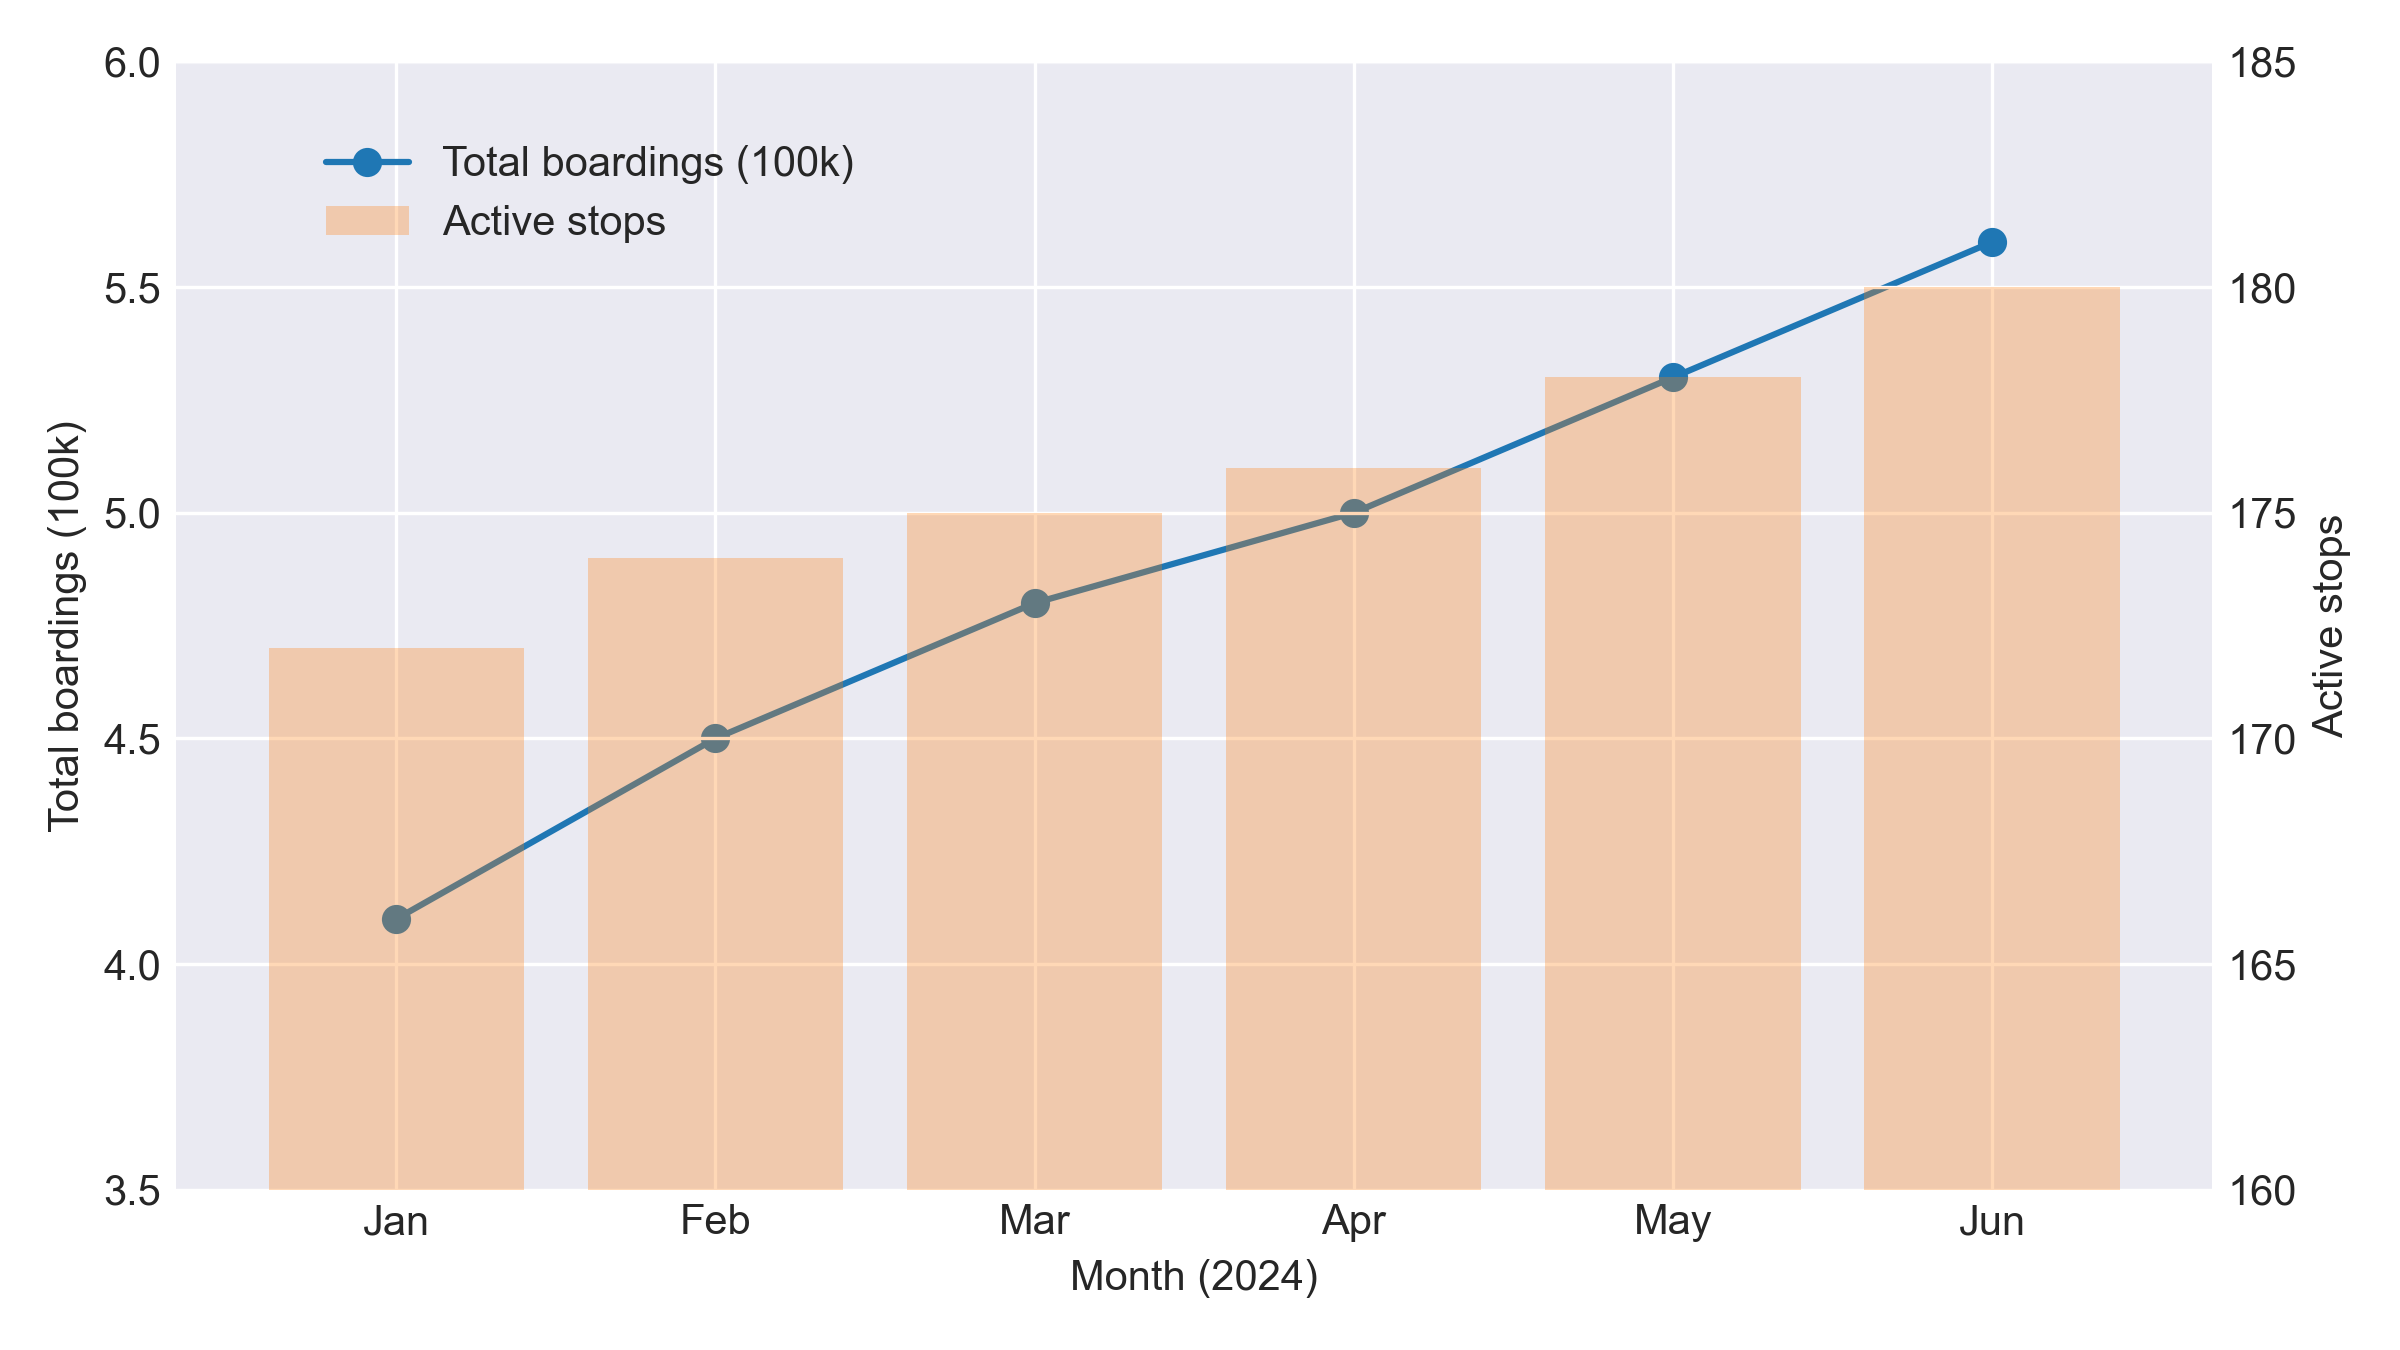
\includegraphics[width=0.82\textwidth]{real_dataset_overview.png}
  \end{center}
  \vspace{0.4em}
  {\small Synthetic Astana dataset: 374 stops, 1.3M boarding records, 12-month coverage.}
\end{frame}

\begin{frame}{Dataset Features (table)}
  \centering
  \small
  \begin{tabular}{p{0.36\textwidth} p{0.56\textwidth}}
    \toprule
    Feature & Description \\
    \midrule
    Boarding count & Target: aggregated boardings per station per period \\
    Weather & Temperature, precipitation, wind speed \\
    Temporal encodings & Hour/day/holiday flags (sine/cosine) \\
    Route metadata & Stop degree, route ID, inbound/outbound \\
    Historical windows & 72-step context (up to 72 hours) \\
    \bottomrule
  \end{tabular}
\end{frame}

\begin{frame}{LA CMTA — Cross-city Validation (visual)}
  \begin{center}
    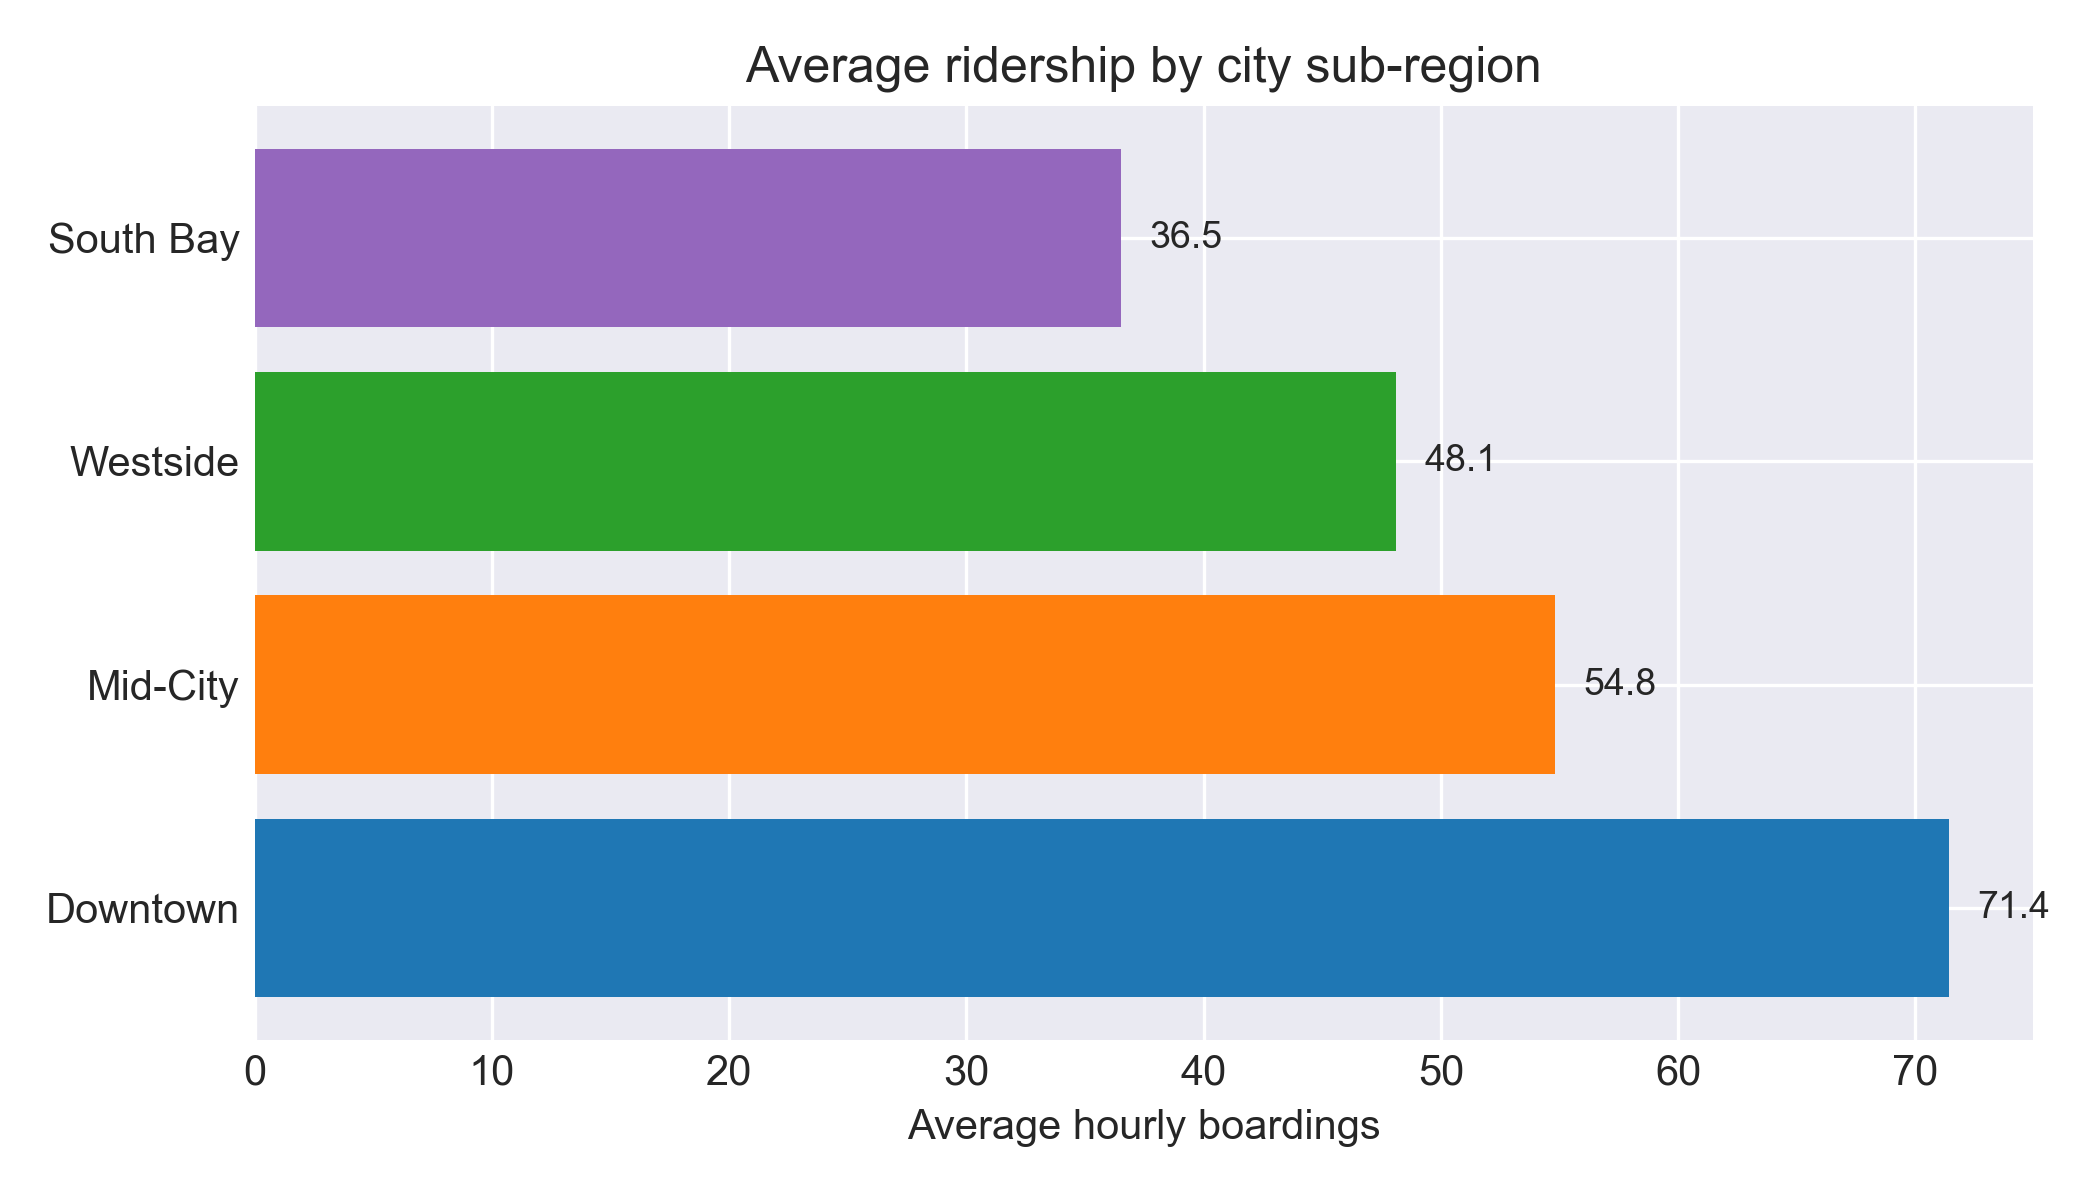
\includegraphics[width=0.82\textwidth]{real_dataset_district_flow.png}
  \end{center}
  \vspace{0.3em}
  {\small LACMTA aggregated features; $R^{2}=0.862$ on held-out districts.}
\end{frame}

% --- Slide 14: Main Results - Scientific & Practical --------------------
\begin{frame}{Main Results of the Research}
  \textbf{Scientific Result:}
  \begin{itemize}
    \item \textbf{$R^{2} = 0.978 \pm 0.001$} \quad MAE $= 11.65 \pm 0.14$ across 42 series (3 seeds).
    \item Outperforms 10 baselines (HA, LSTM, TCN, STGCN, GraphWaveNet, AGCRN).
    \item Ablation: Graph $+0.254\,R^2$ \quad Attention $+0.066\,R^2$
    \item NB calibration: 50\% coverage $= 0.72$, 90\% $= 0.97$ (Poisson severely under-covers).
    \item Cross-city: $R^{2} = 0.862$, MAE $= 7.1$ on LACMTA.
  \end{itemize}

  \vspace{0.3em}
  \textbf{Practical Result:}
  \begin{itemize}
    \item Inference \textbf{$<5$ ms/sample} \quad Parameters: \textbf{542K (2.2 MB)}
    \item LoRA reduces trainable params by \textbf{$94\%$}
    \item Retains \textbf{$R^{2} > 0.95$} under 30\% dropout and moderate noise.
  \end{itemize}
\end{frame}

% --- Slide 15: Research Results (Detailed) ------------------------------
\begin{frame}{Research Results -- Performance Comparison}
  \centering
  \small
  \begin{tabular}{lcccc}
    \toprule
    Method & $R^{2}$ & MAE & RMSE & MAPE ($>5$) \\
    \midrule
    Historical Average & 0.564 & 47.64 & 90.63 & 83.7\% \\
    Seasonal Naive    & 0.551 & 51.97 & 91.98 & 104.6\% \\
    Moving Average    & 0.550 & 51.97 & 92.03 & 104.0\% \\
    \midrule
    LSTM     & 0.696 & 6.33 & 9.69 & 36.1\% \\
    GRU      & 0.697 & 6.32 & 9.67 & 36.0\% \\
    TCN      & 0.697 & 6.33 & 9.66 & 36.1\% \\
    \midrule
    STGCN         & 0.186 & 12.23 & 17.02 & 58.2\% \\
    Graph WaveNet & 0.711 & 6.45  & 10.13 & 35.2\% \\
    AGCRN         & 0.718 & 6.43  & 10.01 & 34.7\% \\
    \midrule
    \textbf{DTS-GSSF (ours)} & \textbf{\color{accent}0.978} & \textbf{\color{accent}11.65} & \textbf{\color{accent}20.54} & \textbf{\color{accent}28.1\%} \\
    \bottomrule
  \end{tabular}

  \vspace{0.2em}
  {\small Evaluated on 42 series; GNN baselines on bottom 28 stations.}
\end{frame}

% --- Visuals for Results ------------------------------------------------
\begin{frame}{Model Comparison — $R^{2}$ (selected)}
  \centering
  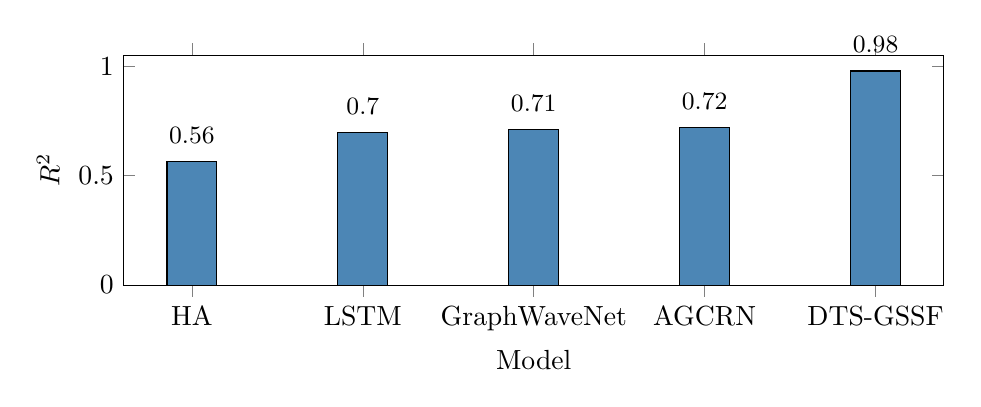
\begin{tikzpicture}
    \begin{axis}[ybar,bar width=18pt, ymin=0, ymax=1.05, width=12cm, height=4.5cm,
      xlabel=Model, ylabel={$R^{2}$}, xtick=data, 
      symbolic x coords={HA,LSTM,GraphWaveNet,AGCRN,DTS-GSSF},
      nodes near coords, nodes near coords style={font=\small, yshift=3pt}]
      \addplot[fill=accent!70] coordinates {(HA,0.564) (LSTM,0.696) (GraphWaveNet,0.711) (AGCRN,0.718) (DTS-GSSF,0.978)};
    \end{axis}
  \end{tikzpicture}
  \vspace{0.3em}
  {\small Representative $R^{2}$ values from evaluation.}
\end{frame}

\begin{frame}{Training Dynamics}
  \begin{center}
    
\includegraphics[width=0.82\textwidth]{training_curves.png}
  \end{center}
  \vspace{0.3em}
  {\small Training loss and validation metrics across epochs.}
\end{frame}

\begin{frame}{Per-Horizon Accuracy}
  \begin{center}
    
\includegraphics[width=0.82\textwidth]{horizon_accuracy.png}
  \end{center}
  \vspace{0.3em}
  {\small Consistent performance across 15, 30, 60, and 120-minute horizons.}
\end{frame}

\begin{frame}{Feature Importance}
  \begin{center}
    
\includegraphics[width=0.82\textwidth]{feature_importance.png}
  \end{center}
  \vspace{0.3em}
  {\small Integrated Gradients attribution: weather dominates prediction.}
\end{frame}

\begin{frame}{Uncertainty Calibration}
  \begin{center}
    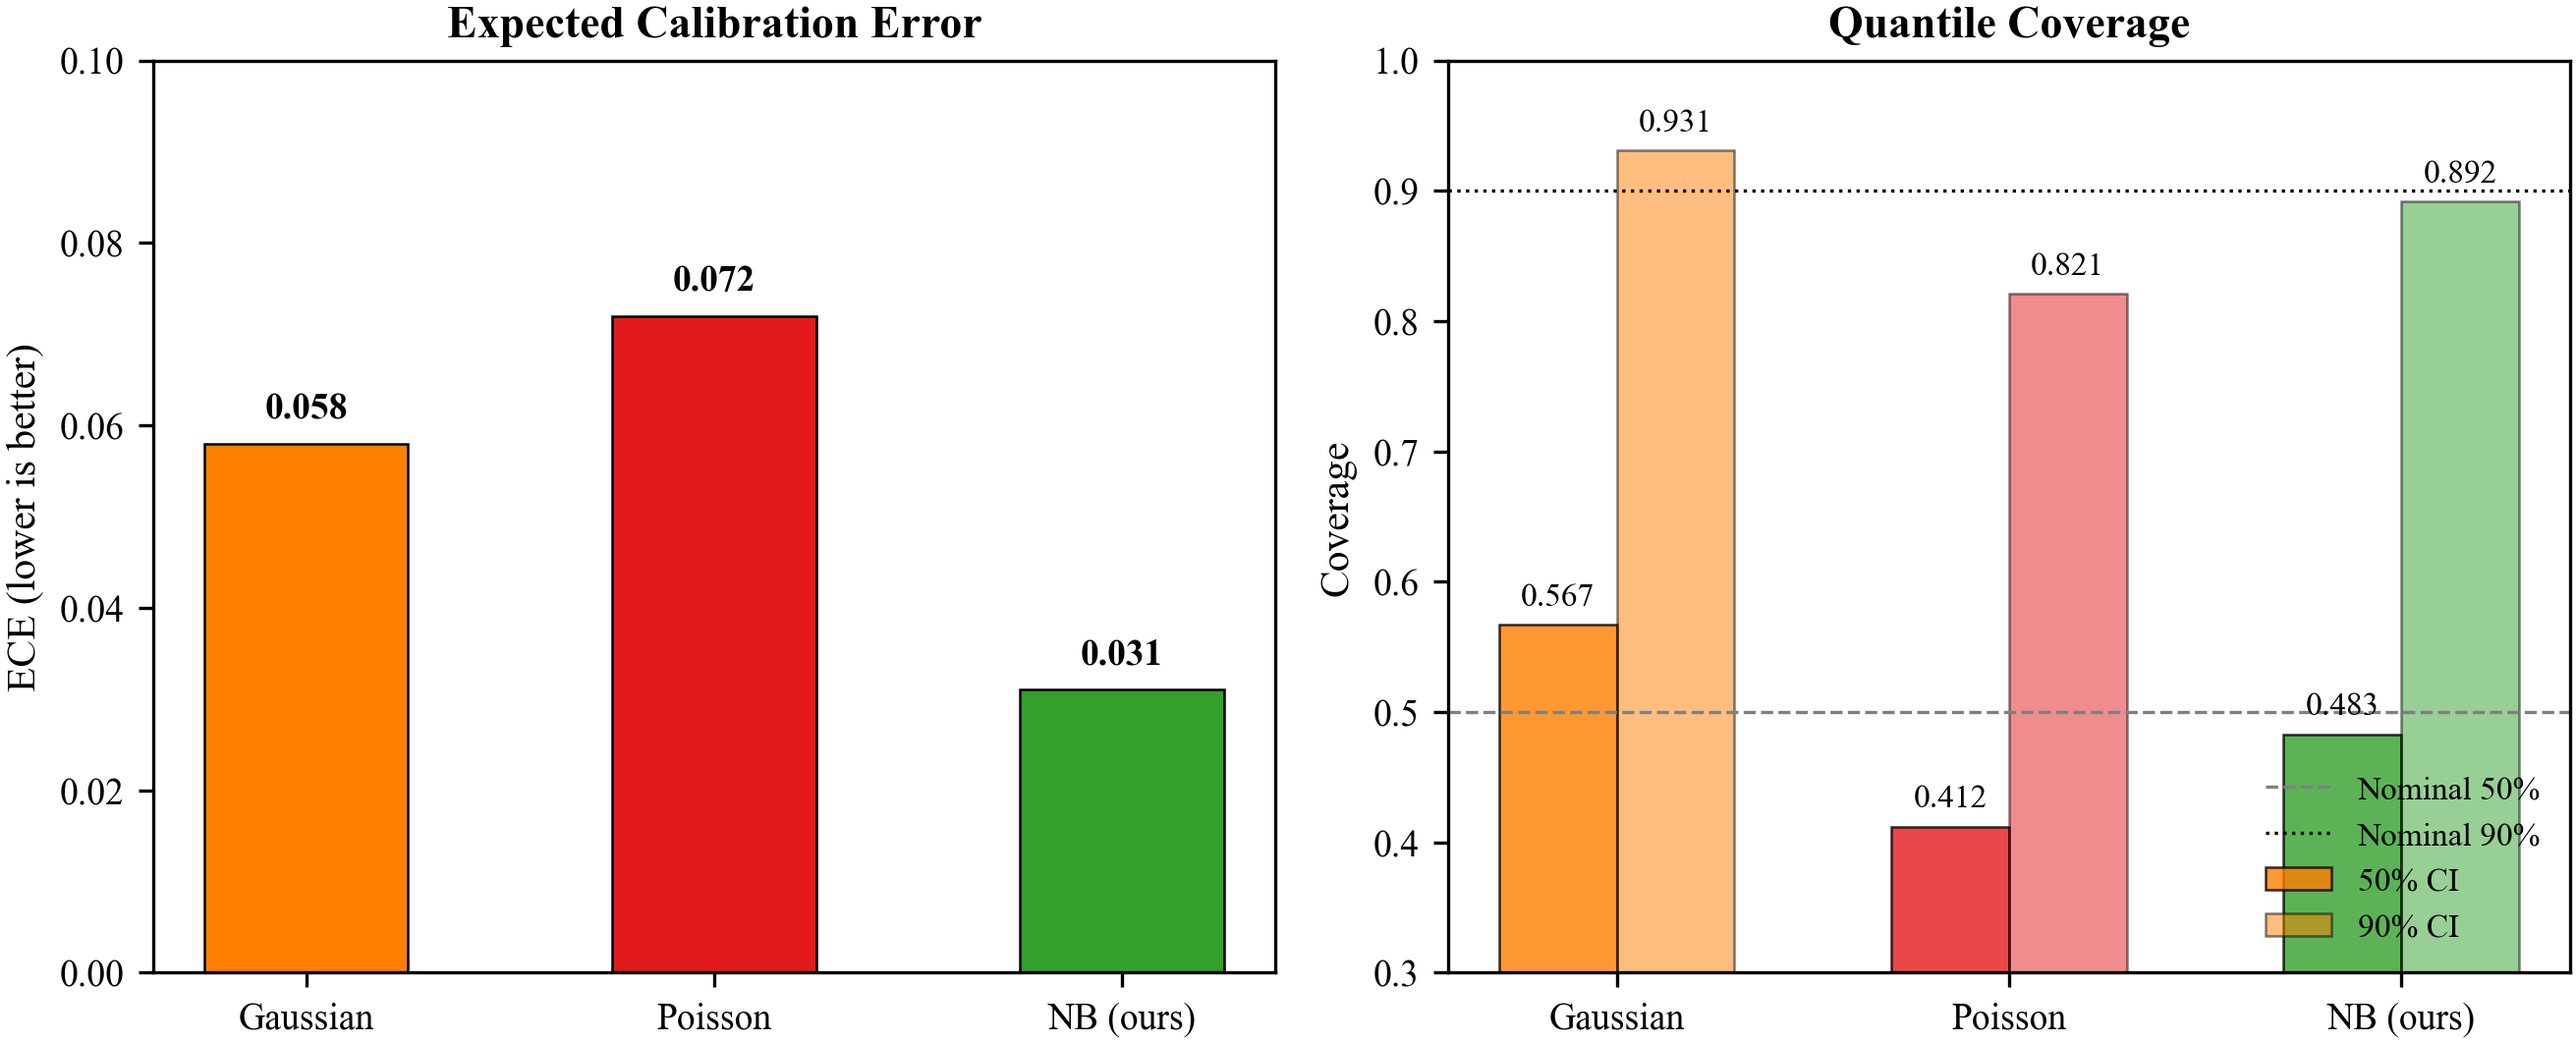
\includegraphics[width=0.82\textwidth]{calibration.png}
  \end{center}
  \vspace{0.3em}
  {\small NB likelihood provides reliable coverage vs. Poisson under-coverage.}
\end{frame}

% --- Slide 21: Additional Results ---------------------------------------
\begin{frame}{Additional Results}
  \textbf{Ablation Study:}
  \begin{itemize}
    \item GRE only: $R^{2} = 0.724$ \quad +Graph: $0.912$ \quad Full: $\mathbf{0.978}$
    \item Physical only ($\alpha=1$): $0.954$ \quad Adaptive only ($\alpha=0$): $0.937$
  \end{itemize}

  \vspace{0.2em}
  \textbf{Per-Horizon Accuracy:}
  \begin{itemize}
    \item Stable $R^{2} = 0.978$ across all horizons \quad MAE range: $11.61$--$11.67$
  \end{itemize}

  \vspace{0.2em}
  \textbf{Feature Attribution:}
  \begin{itemize}
    \item Temperature: \textbf{0.47}, Precipitation: \textbf{0.20}, Cyclical: \textbf{0.12}
    \item \textcolor{accent}{Weather is the dominant ridership predictor.}
  \end{itemize}
\end{frame}

% --- Slide 22: Additional -- Robustness & Computational Cost -----------
\begin{frame}{Robustness \& Computational Cost}
  \textbf{Robustness Analysis:}
  \begin{itemize}
    \item 10\% dropout: $R^{2} = 0.974$ \quad 30\% dropout: $0.951$
    \item Noise $\sigma=0.2$: $R^{2} = 0.971$ \quad 6h gap: $R^{2} = 0.963$
    \item Model retains \textbf{$R^{2} > 0.95$} under all perturbations.
  \end{itemize}

  \vspace{0.4em}
  \textbf{Computational Cost:}
  \centering
  \small
  \begin{tabular}{lccc}
    \toprule
    Method & Train (min) & Inference (ms) & Parameters \\
    \midrule
    LSTM          & 22 & 1.5 & 152K \\
    GRU           & 19 & 0.9 & 39K \\
    STGCN         & 38 & 2.2 & 156K \\
    Graph WaveNet & 62 & 3.0 & 294K \\
    AGCRN         & 78 & 3.5 & 312K \\
    \textbf{DTS-GSSF} & \textbf{\color{accent}14} & \textbf{\color{accent}$<$5} & \textbf{\color{accent}542K} \\
    \bottomrule
  \end{tabular}
\end{frame}

% --- Slide 23: Conclusions per Task -------------------------------------
\begin{frame}{Conclusions per Task (RQ1--RQ5)}
  \small
  \textbf{RQ1 -- Temporal Modelling:} GRE + Attention achieves $R^{2}=0.978$ with stable 72h gradients.\\
  \textbf{RQ2 -- Spatial Modelling:} Dual-adjacency fusion ($\alpha \approx 0.58$) significantly outperforms single-graph setups.\\
  \textbf{RQ3 -- Uncertainty:} NB likelihood delivers calibrated coverage (50\%: 0.72, 90\%: 0.97).\\
  \textbf{RQ4 -- Efficiency:} Sub-5ms inference, 2.2MB size, LoRA cuts trainable params by $94\%$.\\
  \textbf{RQ5 -- Generalisation:} Consistent across horizons; $R^{2}=0.862$ on LACMTA cross-city data.
\end{frame}

% --- Slide 24: Conclusion -----------------------------------------------
\begin{frame}{Conclusion}
  \begin{itemize}
    \item DTS-GSSF achieves \textbf{$R^{2} = 0.978$} and \textbf{MAE $= 11.65$} on Astana's bus network.
    \item \textbf{Key innovations:} Adaptive adjacency + NB uncertainty + LoRA efficiency.
    \item Weather features drive prediction; cyclical patterns contribute 12\%.
    \item Validated cross-city ($R^{2}=0.862$) and robust to dropout/noise ($R^{2}>0.95$).
    \item \textbf{Future work:} Multi-modal transit, dynamic graphs, causal inference, real-world deployment.
  \end{itemize}
\end{frame}

\end{document}